\documentclass{article}
\usepackage{tikz}
\usetikzlibrary{arrows.meta,positioning,calc,shapes.geometric}
\pagestyle{empty}
\begin{document}
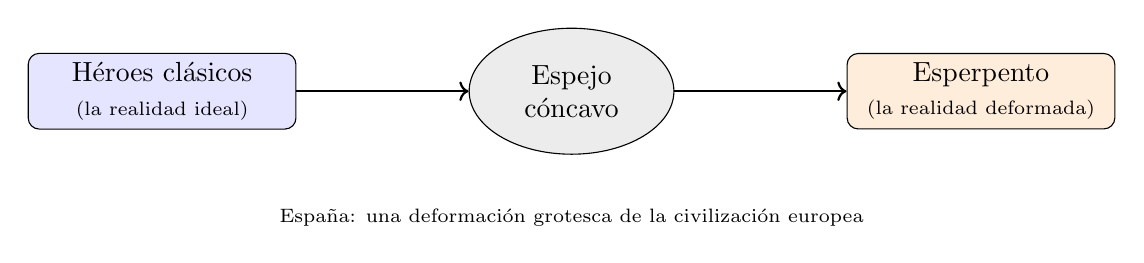
\begin{tikzpicture}
\tikzset{every node/.append style={align=center}}

\node[draw, rounded corners, fill=blue!10, minimum width=3.4cm, align=center] (h) at (0,0) {Héroes clásicos\\ \scriptsize (la realidad ideal)};
\node[draw, ellipse, fill=gray!15, minimum width=2.6cm, minimum height=1.6cm, align=center] (e) at (5.2,0) {Espejo\\ cóncavo};
\node[draw, rounded corners, fill=orange!14, minimum width=3.4cm, align=center] (s) at (10.4,0) {Esperpento\\ \scriptsize (la realidad deformada)};
\draw[->, thick] (h) -- (e); \draw[->, thick] (e) -- (s);
\node[font=\scriptsize, align=center] at (5.2,-1.6) {España: una deformación grotesca de la civilización europea};

\end{tikzpicture}
\end{document}
